% Drawing 142/06-3 -- folder 142, batch 06, archive page 105 (PDF page 106).
% Transcription: Troisième figure, biffée de traits en zigzag : cercles autour de $\infty$, $0$, $1$, un chemin de $1$ vers $\infty$ et un de $0$ vers $1$ ; au-dessus, « 1 cas ».
% Kind: quiver on the sphere minus three points, struck. Method 2 (schematic redraw from the facsimile). Status: ok.
% Notes: Struck through with zigzag strokes (drawn grey, style struck): circles round infinity, 1 (top) and 0 (bottom left), a path from 1 to infinity and one from 0 round to 1. "1 cas" above. The zigzag itself is drawn schematically.
% Coordinates: 1 unit = 1 mm = 1/100 of the crop width (bbox in page fractions: [0.164, 0.237, 0.5, 0.39]).
% Redrawn by Claude (claude-opus-5-5), issue #73, 2026-11-07; not checked by a human; not compiled (no TeX in the session).
% Rights: reproduces part of the work -- behind RENDER_TRANSCRIPTS, never published by itself.
\documentclass[tikz,border=3pt]{standalone}
\usepackage{amsmath,amssymb}
\usetikzlibrary{patterns,arrows.meta}
\tikzset{pencil/.style={black!45}, struck/.style={black!35}, mark/.style={circle,draw,inner sep=1.3pt}, pt/.style={circle,fill,inner sep=0.9pt}, opt/.style={circle,draw,fill=white,inner sep=1.1pt}}
\begin{document}
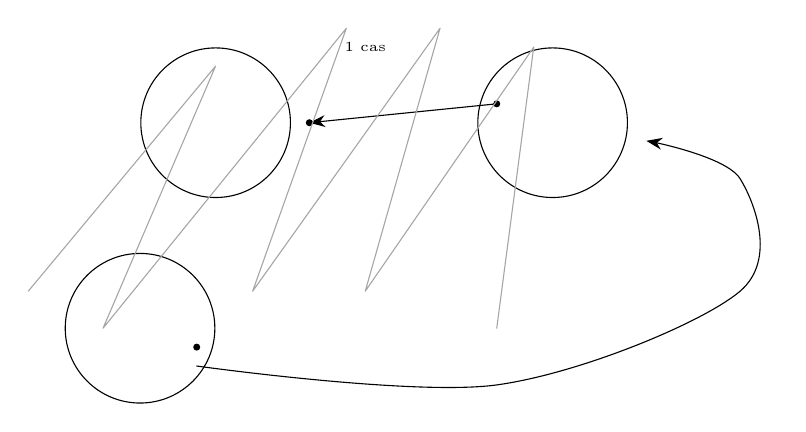
\begin{tikzpicture}[x=1mm,y=1mm,line cap=round,line join=round,font=\scriptsize]
\draw (28.6,-19.1) circle[radius=9.5];
\draw (71.4,-19.1) circle[radius=9.5];
\draw (19,-45.2) circle[radius=9.5];
\node[pt] at (40.5,-19.1) {};
\node[pt] at (64.3,-16.7) {};
\node[pt] at (26.2,-47.6) {};
\draw[-{Stealth[length=2mm]}] (64.3,-16.7) -- (40.5,-19.1);
\draw[-{Stealth[length=2mm]}] plot[smooth, tension=0.55] coordinates {(26.2,-50) (64.3,-52.4) (95.2,-40.5) (95.2,-26.2) (83.3,-21.4)};
\draw[struck] (4.8,-40.5) -- (28.6,-11.9) -- (14.3,-45.2) -- (45.2,-7.1) -- (33.3,-40.5) -- (57.1,-7.1) -- (47.6,-40.5) -- (69,-9.5) -- (64.3,-45.2);
\node[inner sep=1pt] at (47.6,-9.5) {\tiny 1 cas};
\end{tikzpicture}
\end{document}
